\documentclass[8pt]{beamer}
\usepackage{graphicx}
\usepackage{tikz}
\usepackage{lmodern}
\usepackage{mathtools}
\usepackage{minted}
\usepackage[backend=biber]{biblatex}

\usetheme{CambridgeUS}
\usecolortheme{seahorse}
\setbeamercovered{dynamic}
\usefonttheme{professionalfonts}
\setbeamertemplate{itemize items}[default]
\setbeamertemplate{caption}{\raggedright\insertcaption\par}
\bibliography{bibliography.bib}
\newcommand*{\boxedcolor}{red}
\setcounter{tocdepth}{2}

\begin{document}

\title[Compact finite differences on GPUs]
{A novel approach to evaluating 
compact finite differences 
and similar tridiagonal schemes on GPU-accelerated clusters}

\author[Ashwin Srinath]{
        Ashwin Srinath\\
        Department of Mechanical Engineering\\
        \today}
\date{}
\titlepage

\begin{frame}{Overview}
    \tableofcontents
\end{frame}


\section{Motivation}

\begin{frame}
\frametitle{Introduction}
DNS: An approach for numerically solving
the Navier-Stokes equations
\begin{itemize}
\item Extremely fine computational grids
\item High-order accurate numerical schemes
\item e.g., \emph{compact} finite
    difference schemes for approximating derivatives
\item High computational cost
    \begin{itemize}
    \item Feasible only for simple flows
    \item Parallelism almost always required
    \end{itemize}
\end{itemize}
\end{frame}

\begin{frame}
\frametitle{Compact finite difference schemes}
A class of high-order accurate finite difference schemes
for evaluating spatial derivatives

\centering
\includegraphics[width=200px]{img/discretize-function.eps}

\begin{itemize}
\item {General form of compact schemes:
\begin{align*}
\begin{split}
f_i^{\prime} + \alpha(f^{\prime}_{i-1} + f^{\prime}_{i+1}) + \
\beta(f^{\prime}_{i-2} + f^{\prime}_{i+2}) + \hdots  = \
a\frac{f_{i+1} - f_{i-1}}{dx} + \\
b\frac{f_{i+2} - f_{i-2}}{dx} + \
c\frac{f_{i+3} - f_{i-3}}{dx} + \
    \hdots
\end{split}
\end{align*}}
\item $\alpha$, $\beta$, $a$, $b$, $\hdots$ must
    satisfy certain constraints
\item Derivative defined \emph{implicitly}
\end{itemize}
\end{frame}

\begin{frame}
\footnotesize
Solution strategy
\begin{itemize}
\item {Consider the specific scheme:
\begin{align*}
f_i^{\prime} + \frac{1}{4}(f^{\prime}_{i-1} + f^{\prime}_{i+1}) = \
\frac{3}{4}\frac{f_{i+1} - f_{i-1}}{dx}
\end{align*}}

\item {We write the expression for all points:
\begin{align*}
f_2^{\prime} + \frac{1}{4}(f^{\prime}_{1} + f^{\prime}_{3}) =
    \frac{3}{4}\frac{f_{3} - f_{1}}{dx} \\
%
f_3^{\prime} + \frac{1}{4}(f^{\prime}_{2} + f^{\prime}_{4}) =
    \frac{3}{4}\frac{f_{4} - f_{2}}{dx} \\
%
f_4^{\prime} + \frac{1}{4}(f^{\prime}_{3} + f^{\prime}_{5})
    = \frac{3}{4}\frac{f_{5} - f_{3}}{dx} \\
%
\hdots
%
f_{n-1}^{\prime} + \frac{1}{4}(f^{\prime}_{n-2} + f^{\prime}_{n})
    = \frac{3}{4}\frac{f_{n} - f_{n-2}}{dx}
\end{align*}}

\item {Special ``one-sided'' equations are needed near the boundaries:

\begin{align*}
f^{\prime}_1 + 2f^{\prime}_2 &= \frac{-5f_1 + 4f_2 + f_3}{dx} \\
%
f^{\prime}_{n} + 2f^{\prime}_{n-1}
&=
\frac{5f_{n} - 4f_{n-2} -  f_{n-1}}{dx}
\end{align*}}

\end{itemize}
\end{frame}

\begin{frame}[t]
\footnotesize
The full set of equations is expressed succinctly as:
\begin{equation*}
 \begin{bmatrix}
     1&2\\
     1/4&1&1/4\\
     &1/4&1&1/4\\
     &&1/4&1&1/4\\
     &&&1/4&1&1/4\\
     &&&&&\ddots\\
     &&&&&&\ddots\\
     &&&&&&&\ddots\\
     &&&&&&&2&1
  \end{bmatrix}
  \boxed{
  \begin{bmatrix}
      f^{\prime}_1 \\
      f^{\prime}_2 \\
      f^{\prime}_3 \\
      \vdots \\
      \vdots \\
      \vdots \\
      \vdots \\
      f^{\prime}_{n-1} \\
      f^{\prime}_n
   \end{bmatrix}
   }
 =
 \begin{bmatrix}
     \frac{-5f_1 + 4f_2 + f_3}{2dx}\\
     \frac{3(f_{3} - f_{1})}{4dx}\\
     \frac{3(f_{4} - f_{2})}{4dx}\\
     \vdots\\
     \vdots\\
     \vdots\\
     \vdots\\
     \frac{3(f_{n} - f_{n-2})}{4dx}\\
     \frac{5f_{n} - 4f_{n-1} - f_{n-2}}{2dx}
  \end{bmatrix}
\end{equation*}

Solution yields the derivatives at all points
$i=1,2, \hdots n$ simultaneously.
\begin{itemize}
\item In general, compact schemes yield banded systems
\item Tridiagonal schemes generally sufficient
\end{itemize}
\end{frame}

\begin{frame}
\frametitle{Objectives}
\begin{itemize}
    \item Exploratory work for exploiting GPUs
        in current research code
        \begin{itemize}
            \item important step for our group: Palmetto cluster
        currently has 598 GPUs (and counting)
        \end{itemize}
    \item An efficient GPU tridiagonal solver
    \item Parallelize the compact finite difference evaluation---current
        research code uses a sequential approach
\end{itemize}
\end{frame}

\begin{frame}
\frametitle{Thesis contributions}
\begin{itemize}
    \item A novel solution strategy for
        the tridiagonal systems arising in
        compact finite differences
        and other numerical schemes
    \item A strategy for evaluating compact
        finite differences on GPU-accelerated clusters
\end{itemize}
\end{frame}


\section{Background}

\subsection{Compact finite difference schemes}

\begin{frame}
\frametitle{Evaluation of spatial derivatives}
\pause
\centering
\includegraphics[width=200px]{img/discretize-function.eps}
\begin{itemize}[<+->]
    \item {Explicit schemes express
        the derivative \emph{explicitly}
        in terms of function values:
        \begin{equation*}
            f_i^\prime = \frac{f_{i+1} - f_{i-1}}{2dx}
        \end{equation*}
        }
    \item {Compact schemes express
        the derivative \emph{implicitly}:
        \begin{equation*}
            f_i^{\prime} + \frac{1}{4}(f^{\prime}_{i-1} + f^{\prime}_{i+1}) = \
            \frac{3}{4}\frac{f_{i+1} - f_{i-1}}{dx}
        \end{equation*}
        }
    \item Given the function values,
        easy to compute the derivative using explicit schemes
    \begin{itemize}
        \item easily parallelized
    \end{itemize}
\end{itemize}
\end{frame}

\begin{frame}
For compact schemes,
we write the expression for all points:

\begin{align*}
f_2^{\prime} + \frac{1}{4}(f^{\prime}_{1} + f^{\prime}_{3}) =
    \frac{3}{4}\frac{f_{3} - f_{1}}{dx} \\
%
f_3^{\prime} + \frac{1}{4}(f^{\prime}_{2} + f^{\prime}_{4}) =
    \frac{3}{4}\frac{f_{4} - f_{2}}{dx} \\
%
f_4^{\prime} + \frac{1}{4}(f^{\prime}_{3} + f^{\prime}_{5})
    = \frac{3}{4}\frac{f_{5} - f_{3}}{dx} \\
%
\hdots
%
f_{n-1}^{\prime} + \frac{1}{4}(f^{\prime}_{n-2} + f^{\prime}_{n})
    = \frac{3}{4}\frac{f_{n} - f_{n-2}}{dx}
\end{align*}

- special ``one-sided'' equations are needed near the boundaries:

\begin{align*}
f^{\prime}_1 + 2f^{\prime}_2 &= \frac{-5f_1 + 4f_2 + f_3}{dx} \\
%
f^{\prime}_{n} + 2f^{\prime}_{n-1}
&=
\frac{5f_{n} - 4f_{n-2} -  f_{n-1}}{dx}
\end{align*}
\end{frame}

\begin{frame}
\onslide<1->{The full set of equations is expressed succinctly as:}

\only<1>{
\begin{equation*}
 \begin{bmatrix}
     1&2\\
     1/4&1&1/4\\
     &1/4&1&1/4\\
     &&1/4&1&1/4\\
     &&&1/4&1&1/4\\
     &&&&&\ddots\\
     &&&&&&\ddots\\
     &&&&&&&\ddots\\
     &&&&&&&2&1
  \end{bmatrix}
  \begin{bmatrix}
      f^{\prime}_1 \\
      f^{\prime}_2 \\
      f^{\prime}_3 \\
      \vdots \\
      \vdots \\
      \vdots \\
      \vdots \\
      f^{\prime}_{n-1} \\
      f^{\prime}_n
   \end{bmatrix}
 =
 \begin{bmatrix}
     \frac{-5f_1 + 4f_2 + f_3}{2dx}\\
     \frac{3(f_{3} - f_{1})}{4dx}\\
     \frac{3(f_{4} - f_{2})}{4dx}\\
     \vdots\\
     \vdots\\
     \vdots\\
     \vdots\\
     \frac{3(f_{n} - f_{n-2})}{4dx}\\
     \frac{5f_{n} - 4f_{n-1} - f_{n-2}}{2dx}
  \end{bmatrix}
\end{equation*}
}

\only<2>{
\begin{equation*}
 \begin{bmatrix}
     1&2\\
     1/4&1&1/4\\
     &1/4&1&1/4\\
     &&1/4&1&1/4\\
     &&&1/4&1&1/4\\
     &&&&&\ddots\\
     &&&&&&\ddots\\
     &&&&&&&\ddots\\
     &&&&&&&2&1
  \end{bmatrix}
  \boxed{
  \begin{bmatrix}
      f^{\prime}_1 \\
      f^{\prime}_2 \\
      f^{\prime}_3 \\
      \vdots \\
      \vdots \\
      \vdots \\
      \vdots \\
      f^{\prime}_{n-1} \\
      f^{\prime}_n
   \end{bmatrix}
   }
 =
 \begin{bmatrix}
     \frac{-5f_1 + 4f_2 + f_3}{2dx}\\
     \frac{3(f_{3} - f_{1})}{4dx}\\
     \frac{3(f_{4} - f_{2})}{4dx}\\
     \vdots\\
     \vdots\\
     \vdots\\
     \vdots\\
     \frac{3(f_{n} - f_{n-2})}{4dx}\\
     \frac{5f_{n} - 4f_{n-1} - f_{n-2}}{2dx}
  \end{bmatrix}
\end{equation*}
}

\onslide<2> {Solution yields the derivatives at all points
$i=1,2, \hdots n$ simultaneously.}

\end{frame}

\begin{frame}
    \begin{itemize}
    \item {General form of compact schemes:
    \begin{align*}
        \begin{split}
            f_i^{\prime} + \alpha(f^{\prime}_{i-1} + f^{\prime}_{i+1}) + \
            \beta(f^{\prime}_{i-2} + f^{\prime}_{i+2}) + \hdots  = \
            a\frac{f_{i+1} - f_{i-1}}{dx} + \\
            b\frac{f_{i+2} - f_{i-2}}{dx} + \
            c\frac{f_{i+3} - f_{i-3}}{dx} + \
            \hdots
        \end{split}
    \end{align*}}
    \item In general, yield \emph{banded} linear systems
    \item Tridiagonal schemes ($\beta=0$) are generally sufficient
    \end{itemize}
\end{frame}


\iffalse
\begin{frame}
\frametitle{Finite difference methods}
\pause
\begin{itemize}[<+->]
    \item <2-> Method for solving ordinary and
        partial differential equations
    \item <3-> Approximates the derivatives
        appearing in the equations
        by \emph{finite-difference} approximations
    \item <4-> Two types of derivatives:
    \begin{itemize}
        \item <5-> Spatial
        \item <6-> Temporal
    \end{itemize}
\end{itemize}

\onslide<4-> {
\begin{equation*}
    \alert<6>{\frac{\partial T}{\partial t}} = \alpha (\alert<5>{\frac{\partial^2 T}{\partial x^2}} + \
        \alert<5>{\frac{\partial^2 T}{\partial y^2}})
\end{equation*}
}
\end{frame}

\begin{frame}[t]
\frametitle{Finite difference approximation}
Finite difference approximation of the
first derivative of a uniformly sampled function
\begin{figure}
\includegraphics[width=120px]{img/discretize-function.eps}
\caption{Function $f(x)$, sampled with sampling width $dx$}
\end{figure}
\end{frame}

\begin{frame}[t]
\frametitle{Finite difference approximation}
At sample point $i$,
various approaches for approximating the first derivative:
\begin{columns}[c]
\visible<2->{
    \begin{column}[T]{3cm}
    \begin{figure}
    \includegraphics[width=100px]{img/forward-difference.eps}
    \caption{\textbf{Forward difference}:
        derivative expressed in terms of function values
        at $i$, $i+1$, $i+2$, $\hdots$
    }
    \end{figure}
    \end{column}
}

\visible<3->{
    \begin{column}[T]{3cm}
    \begin{figure}
    \includegraphics[width=100px]{img/backward-difference.eps}
    \caption{\textbf{Backward difference}:
        derivative expressed in terms of function values
        at $\hdots$, $i-2$, $i-1$, $i$
    }
    \end{figure}
    \end{column}
}

\visible<4->{
    \begin{column}[T]{3cm}
    \begin{figure}
    \includegraphics[width=100px]{img/central-difference.eps}
    \caption{\textbf{Central difference}:
        derivative expressed in terms of function values
        at $\hdots$, $i-2$, $i-1$, $i$, $i+1$, $i+2$, $\hdots$
    }
    \end{figure}
    \end{column}
}
\end{columns}
\end{frame}

\begin{frame}[fragile]
\frametitle{Explicit finite difference schemes}
\pause
\begin{itemize}[<+->]
\item The schemes are \emph{explicit}
    because the derivative at each point $i$
    can be expressed \emph{explicitly}
    as some combination of function values
\item Easy to implement in code:
\end{itemize}
\end{frame}

\begin{frame}[t]
\frametitle{Finite difference stencils}
\footnotesize

\begin{block}
{Second order accurate central finite difference scheme} 
\begin{equation*}
    f_i^\prime = \frac{f_{i+1} - f_{i-1}}{2dx}
\end{equation*}
\centering
\includegraphics[width=150px]{img/second-order-stencil.eps}
\end{block}

\begin{block}
{Fourth order accurate central finite difference scheme}
\begin{equation*}
    f_i^\prime = \frac{-f_{i+2} + 4f_{i+1} - 4f_{i-1} +f_{i-2}}{12dx}
\end{equation*}
\centering
\includegraphics[width=150px]{img/fourth-order-stencil.eps}
\end{block}
\end{frame}

\begin{frame}

\end{frame}


\begin{frame}
\frametitle{Parallel computation of finite differences}
\only<1> {
    One dimensional grid of $n$ points:
    \begin{figure}
    \centering
    \includegraphics[width=200px]{img/long-1d-domain.eps}
    \end{figure}
}
\only<2> {
    Split the domain among two parallel processes:
    \begin{figure}
    \centering
    \includegraphics[width=200px]{img/long-1d-domain-split.eps}
    \end{figure}
}
\only<3> {
    Each process can easily compute the derivative at its ``inner points'':
    \begin{figure}
    \centering
    \includegraphics[width=150px]{img/local-derivative-evaluation-inner.eps}
    \end{figure}
}
\only<4> {
    At the process boundaries, communication may be required:
    \begin{figure}
    \centering
    \includegraphics[width=200px]{img/local-derivative-evaluation-boundary.eps}
    \end{figure}
}
\only<5> {
    For a 2-D domain, communication required at each grid line:
    \begin{figure}
    \centering
    \includegraphics[width=200px]{img/local-derivative-evaluation-boundary-2d.eps}
    \end{figure}
}
\only<6> {
    Amount of communication grows with problem dimensionality and stencil width:
    \begin{figure}
    \centering
    \includegraphics[width=200px]{img/overall-halos.eps}
    \end{figure}
}
\end{frame}

\begin{frame}
\begin{itemize}[<+->]
    \item Explicit finite difference schemes are simple to implement
    \item Higher order accurate schemes require wider stencils
    \item Reduces the compute to communicate ratio in parallel
\end{itemize}
\end{frame}

\begin{frame}
\frametitle{Compact finite difference schemes}
\begin{itemize}[<+->]
    \item High order of accuracy for smaller stencil widths
    \item Express the derivative \emph{implicitly}:
    \item [] \begin{align*}
        \begin{split}
            f_i^{\prime} + \alpha(f^{\prime}_{i-1} + f^{\prime}_{i+1}) + \
            \beta(f^{\prime}_{i-2} + f^{\prime}_{i+2}) + \hdots  = \
            a\frac{f_{i+1} - f_{i-1}}{dx} + \\
            b\frac{f_{i+2} - f_{i-2}}{dx} + \
            c\frac{f_{i+3} - f_{i-3}}{dx} + \
            \hdots
        \end{split}
        \end{align*}
\end{itemize}
\end{frame}

\begin{frame}
\footnotesize
\begin{align*}
\begin{split}
    f_i^{\prime} + \alpha(f^{\prime}_{i-1} + f^{\prime}_{i+1}) + \
    \beta(f^{\prime}_{i-2} + f^{\prime}_{i+2}) + \hdots = \
    a\frac{f_{i+1} - f_{i-1}}{h} + \\
    b\frac{f_{i+2} - f_{i-2}}{h} + \
    c\frac{f_{i+3} - f_{i-3}}{h} + \
    \hdots
\end{split}
\end{align*}
\pause
\begin{itemize}
    \item <2-> Difficult to implement compared to explicit schemes
    \item <3-> Consider the scheme with
        $\alpha=\frac{1}{4}$, $\beta=0$, $a=\frac{3}{4}$,
        $b=c=\hdots=0$:
    \item <4-> For $i = 2, 3, \hdots .. n-1$:
\end{itemize}
\begin{align*}
\onslide<5->{f_2^{\prime} + \frac{1}{4}(f^{\prime}_{1} + f^{\prime}_{3}) =
    \frac{3}{4}\frac{f_{3} - f_{1}}{dx}} \\
%
\onslide<6->{f_3^{\prime} + \frac{1}{4}(f^{\prime}_{2} + f^{\prime}_{4}) =
    \frac{3}{4}\frac{f_{4} - f_{2}}{dx} \\}
%
\onslide<7->{f_4^{\prime} + \frac{1}{4}(f^{\prime}_{3} + f^{\prime}_{5})
    = \frac{3}{4}\frac{f_{5} - f_{3}}{dx} \\}
%
\onslide<8->{\hdots}
\onslide<8->{f_{n-1}^{\prime} + \frac{1}{4}(f^{\prime}_{n-2} + f^{\prime}_{n})
    = \frac{3}{4}\frac{f_{n} - f_{n-2}}{dx}}
\end{align*}
\end{frame}

\begin{frame}
\begin{itemize}
    \item Special equations required to close the boundaries
    \item Boundary equations have the following general form:
        \begin{equation*}
            f_1^{\prime} + \alpha^{\prime}f_2^{\prime} = \
                \frac{1}{h}(a^{\prime}f_1 + b^{\prime}f_2 + \
                    c^{\prime}f_3 + d^{\prime}f_4)
        \end{equation*}
    \item Consider the following boundary scheme 
        \begin{align*}
            f^{\prime}_1 + 2f^{\prime}_2 &= \frac{-5f_1 + 4f_2 + f_3}{dx} \\
            f^{\prime}_{n} + 2f^{\prime}_{n-1}
            &=
            \frac{5f_{n} - 4f_{n-2} -  f_{n-1}}{dx}
        \end{align*}
\end{itemize}
\end{frame}

\begin{frame}
\footnotesize
The full set of equations is:
\begin{align*}
    f^{\prime}_1 + 2f^{\prime}_2 &= \frac{-5f_1 + 4f_2 + f_3}{dx} \\
    %
    f_2^{\prime} + \frac{1}{4}(f^{\prime}_{1} + f^{\prime}_{3}) &=
        \frac{3}{4}\frac{f_{3} - f_{1}}{dx} \\
    %
    f_3^{\prime} + \frac{1}{4}(f^{\prime}_{2} + f^{\prime}_{4}) &=
        \frac{3}{4}\frac{f_{4} - f_{2}}{dx} \\
    %
    f_4^{\prime} + \frac{1}{4}(f^{\prime}_{3} + f^{\prime}_{5}) &=
        \frac{3}{4}\frac{f_{5} - f_{3}}{dx} \\
    %
    \hdots& \\
    %
    f_{n-1}^{\prime} + \frac{1}{4}(f^{\prime}_{n-2} + f^{\prime}_{n}) &=
        \frac{3}{4}\frac{f_{n} - f_{n-2}}{dx} \\
    %
    f^{\prime}_{n} + 2f^{\prime}_{n-1} &=
        \frac{5f_{n} - 4f_{n-2} -  f_{n-1}}{dx}
\end{align*}
\end{frame}

\begin{frame}
\footnotesize
Can be expressed as a system of equations:
\begin{equation*}
 \begin{bmatrix}
     1&2\\
     1/4&1&1/4\\
     &1/4&1&1/4\\
     &&1/4&1&1/4\\
     &&&1/4&1&1/4\\
     &&&&&\ddots\\
     &&&&&&\ddots\\
     &&&&&&&\ddots\\
     &&&&&&&2&1
  \end{bmatrix}
  \begin{bmatrix}
      f^{\prime}_1 \\

      f^{\prime}_2 \\
      f^{\prime}_3 \\
      \vdots \\
      \vdots \\
      \vdots \\
      \vdots \\
      f^{\prime}_{n-1} \\
      f^{\prime}_n
   \end{bmatrix}
 =
 \begin{bmatrix}
     \frac{-5f_1 + 4f_2 + f_3}{2dx}\\
     \frac{3(f_{3} - f_{1})}{4dx}\\
     \frac{3(f_{4} - f_{2})}{4dx}\\
     \vdots\\
     \vdots\\
     \vdots\\
     \vdots\\
     \frac{3(f_{n} - f_{n-2})}{4dx}\\
     \frac{5f_{n} - 4f_{n-1} - f_{n-2}}{2dx}
  \end{bmatrix}
\end{equation*}

\pause
\begin{itemize}[<+->]
    \item The derivatives at $i=1,2, .. n$ are solved \emph{simultaneously}
    \item In general, this requires solution of a \emph{banded} linear system
\end{itemize}
\end{frame}


\begin{frame}
\frametitle{The need for parallel systems}
\pause
\begin{itemize}[<+->]
    \item Computation established as the ``third route''
        to scientific truth
    \item Solving real problems:
        energy research,
        climate modeling,
        protein folding,
        quantum mechanics...
    \item Computational \emph{power} soon becomes
        the bottleneck for the size and scope of
        problems that can be solved
    \item 2003 famously quoted as the end
        of the monolithic processor;
        parallel computing synonymous with
        high-performance computing
\end{itemize}
\end{frame}

\begin{frame}[shrink=20,t]
\frametitle{The workhorses of scientific computation}
\pause
\begin{columns}[T]
\visible<2->{
\begin{column}{0.33\textwidth}
\textbf{Multi-core CPU}
\includegraphics[width=100px]{img/intel-xeon-device.jpg}
\begin{itemize}
    \item<5-> 2-16 cores
    \item<6-> General-purpose computation
    \item<7-> Programming: OpenMP, PThreads, MPI
    \item<8-> Focus of vast majority of scientific
        software
\end{itemize}
\end{column}
}

\visible<3->{
\begin{column}{0.33\textwidth}
\textbf{Many-core GPU}
\includegraphics[width=100px]{img/tesla-k20-device.jpg}
\begin{itemize}
    \item<9-> Hundreds of compute cores
    \item<10-> \emph{Massively-parallel} computations
    \item<11-> Programming: CUDA, OpenCL
    \item<12-> Supported by major packages,
        proven for several applications
\end{itemize}
\end{column}
}

\visible<4->{
\begin{column}{0.33\textwidth}
\textbf{Intel Many Integrated Core \emph{coprocessor}}
\includegraphics[width=120px]{img/xeon-phi-device.png}
\begin{itemize}
    \item<13-> 50-72 cores
    \item<14-> Require more parallelism to reach
        peak performance
    \item<15-> CPU-like programmability
    \item<16-> Support by packages is scarce
        but growing
\end{itemize}
\end{column}
}
\end{columns}
\end{frame}

\begin{frame}[t]
\frametitle{Why GPUs?}
\pause
\footnotesize
\begin{columns}[T]
\begin{column}{0.4\textwidth}
\begin{itemize}
    \item<2-> Higher peak performance
        compared to multicore CPUs
    \item<3-> Higher memory bandwidth
    \item<4-> Devotes more resources
        (transistors) to computing
        rather than caching/control flow
    \item<5-> Well-suited to
        highly data-parallel computations---often the
        \emph{kernels} in scientific computation
\end{itemize}
\end{column}

\begin{column}{0.6\textwidth}
\includegraphics<2>[width=180px]
    {img/floating-point-operations-per-second.png}
\includegraphics<3>[width=180px]
    {img/memory-bandwidth.png}
\includegraphics<4>[width=180px]
    {img/device-comparison.png}
\includegraphics<5>[width=180px]
    {img/device-comparison.png}
\end{column}
\end{columns}
\end{frame}


\section{Proposed Tridiagonal Algorithm}
\begin{frame}
\frametitle{Graphics processing units}
\begin{columns}[c]
\begin{column}[T]{5cm}
    Expectations
    \begin{figure}
    \includegraphics[width=150px]{img/expectations.jpg}
    \end{figure}
\end{column}

\begin{column}[T]{5cm}
    Reality
    \begin{figure}
    \includegraphics[width=150px]{img/reality.png}
    \end{figure}
\end{column}
\end{columns}
\end{frame}

\section{Distributed Compact Finite Difference Evaluation}
\begin{frame}
\frametitle{Graphics processing units}
\begin{columns}[c]
     \begin{column}[T]{5cm}
        Expectations
        \begin{figure}
        \includegraphics[width=150px]{img/expectations.jpg}
        \end{figure}
    \end{column}

    \begin{column}[T]{5cm}
        Reality
        \begin{figure}
        \includegraphics[width=150px]{img/reality.png}
        \end{figure}
    \end{column}
\end{columns}
\end{frame}

\section{Results}

\begin{frame}
\frametitle{Graphics processing units}
\begin{columns}[c]
     \begin{column}[T]{5cm}
        Expectations
        \begin{figure}
        \includegraphics[width=150px]{img/expectations.jpg}
        \end{figure}
    \end{column}

    \begin{column}[T]{5cm}
        Reality
        \begin{figure}
        \includegraphics[width=150px]{img/reality.png}
        \end{figure}
    \end{column}
\end{columns}
\end{frame}
\fi

\end{document}

